Sikteeri on Kapsi ry:n laskutuksen ja jäsenhallinnan tarpeisiin kehitetty web-palvelu. Sen lisäksi yhdistyksellä on käytössä erillinen komentorivityökalu, nimeltä admtool, jolla voidaan tehdä erilaisia ylläpitotehtäviä. Näitä työkaluja pääsevät käyttämään Kapsi ry:n tekninen ylläpito, hallituksen jäsenet ja toimihenkilöt.

Ylläpidon työkalujen nykyinen arkkitehtuuri on kuvattu kuvassa \ref{kapsi_nykyinen}. Sekä Sikteeri että admtool käyttävät ulkoisena komponenttina LDAP-käyt\-tä\-jä\-tie\-to\-kan\-taa, josta tarkistetaan, onko käyttäjällä oikeus käyttää palvelua. Sikteeri ei käytä LDAP-tietokantaa suoraan, vaan sillä on oma SQL-muotoinen käyttäjätietokanta, johon käyttäjätiedot synkronoidaan LDAP:sta. Admtool on taas suoraan yhteydessä LDAP-tietokantaan.

\begin{figure}[h]
\centering
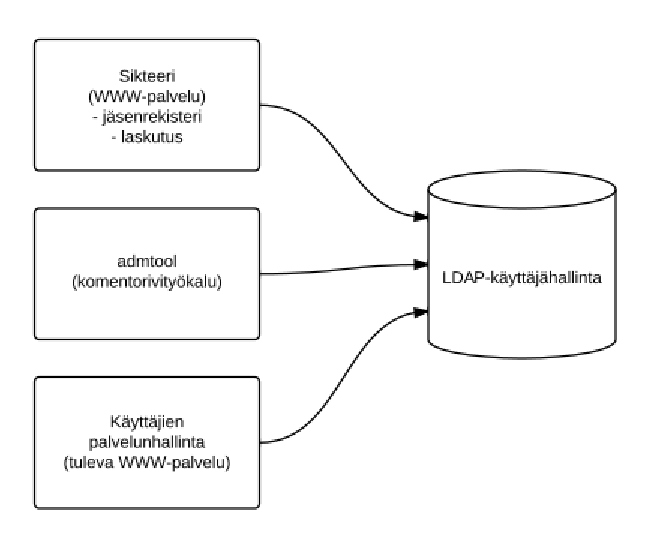
\includegraphics[width=.7\textwidth]{toteutus/kapsi_nykyinen.eps}
\caption{Kapsin jäsenhallintapalveluiden arkkitehtuuri.}%
\label{kapsi_nykyinen}
\end{figure}

Sihteerin on toteutettu Python-kielisellä Django-so\-vel\-lus\-ke\-hyk\-sel\-lä. Käyttäjien tunnistamiseen käytetään sovelluskehyksen tarjoamaa django.contrib.auth-vä\-li\-oh\-jel\-mis\-to\-a, joka tarjoaa hyvät mahdollisuudet arkkitehtuurin laajentamiseen \cite{django_auth}. Väliohjelmistossa on mahdollista määritellä eri taustajärjestelmiä (backend), joita käytetään tunnistautumisessa. Sikteeri käyttää tunnistautumiseen Djangon tarjoamaa ModelBackend-taustajärjestelmää, joka mahdollistaa käyttäjän tunnistamisen vertaamalla käyttäjän syöttämää käyttäjätunnusta ja salasanaa tietokantaan tallennettuihin käyttäjätietoihin \cite{django_auth}. Jos oikealla tunnus/salasana-parilla oleva käyttäjä löytyy, palautetaan käyttäjän tiedot sovellustasolle.

Sikteerin käyttäjillä on siis oma Sikteeri-käyttäjätunnus. Käyttäjän perustiedot on tuotu käyttäjätietokannasta, mutta muutokset eivät siirry Sikteeristä takaisin käyttäjätietokantaan. Tällöin esimerkiksi käyttäjän vaihtaessa Sikteerin salasanan, on hänellä Kapsin sisällä kaksi erillistä tunnus/salasana-paria.